\chapter{Experiment} 
\label{Chapter3} 
\lhead{Chapter 3. \emph{Experiment}} 

This chapter is a comprehensive benchmark of SocketCluster. to begin with, the
scalability of the client code will be checked with a client throughout test.
Then once the the client has been proof checked, the first experiment will
compare SocketCluster and engine.io. 

Then the experiment will purely focus on SocketCluster. The first one will
evaluate the influence of adding more cores on the performances. The second one
will study the influence of external parameters like the period of pings, the
size of the messages and the number of communications. And to finish a
concurrent experiment will be carried out in order to have an idea of
SocketCluster's behavior in highly parallel environment.  

\section{Client throughout}

This first section is composed of two experiment to check the client code is
behaving like expected.

\subsection{Client scalability}

SocketCluster-client makes the instantiation of a WebSocket clients on one core
quite straightforward. To deploy it on all available nodes, node.js
\texttt{fork()} function is used. A client code example is given in appendix
\ref{fig:WS_client_simplePing}.

The first experiment is a safety test. It checks if \texttt{fork()} distributes
evenly the work among the cores.

\begin{center}
  \begin{tabular}{ | l | l |}
  \hline
  \multicolumn{2}{|c|}{Parameters} \\
  \hline
    Instance type &  amazon s3 m3.2xlarge\\ 
    Experiment time & 120 s \\
    Number of new communication created at each iteration & 15 \\
    Client creation period & 1 s \\
    Type of ping & random number \\ 
    Ping period & 2.5 s \\ 
  \hline
  \end{tabular}
\end{center}

\begin{figure}[H]
	\centering
		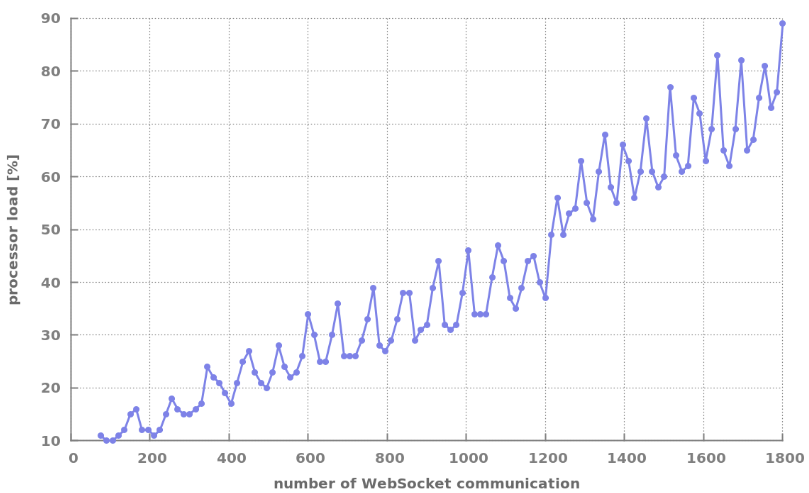
\includegraphics[width=\textwidth]{./Figures/1_client.png}
		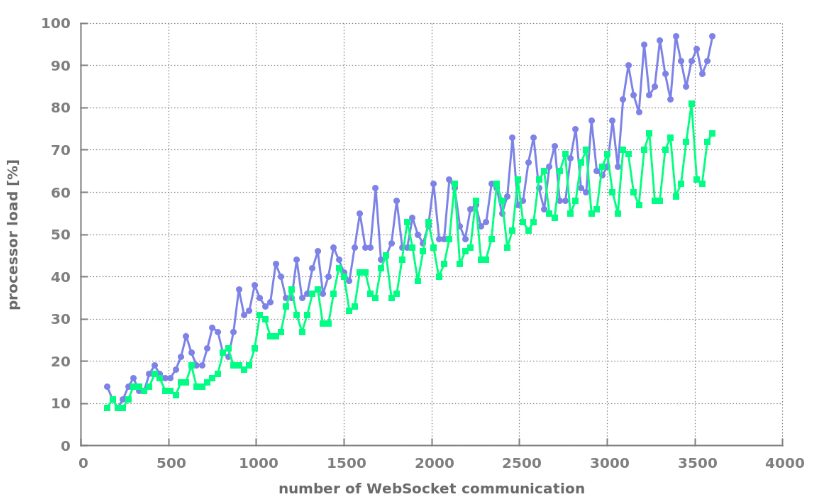
\includegraphics[width=\textwidth]{./Figures/2_client.png}
	\caption[Client throughout]{Client throughout}
	\label{fig:1+2_client}
\end{figure}


From Figure \ref{fig:1+2_client} it can be inferred that the client
implementation works flawlessly. Adding a second core enables twice as much
communication  to be established.

\subsection{browser testing}

As mentioned in Appendix \ref{fig:index_script}, by operating minor changes in
the \texttt{index.html} file, the browser can be configured to display in real
time the number of pings received by a particular worker. If the experiment is
running locally, typing \texttt{localhost:8080} in the url will link the
browser to one worker.

\begin{figure}[H]
	\centering
		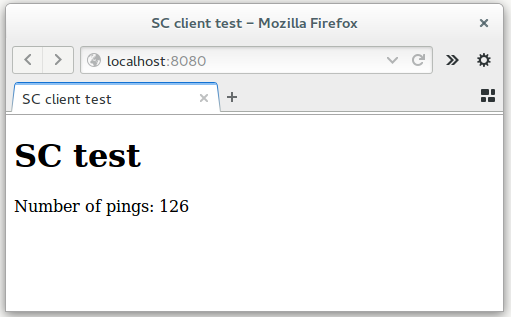
\includegraphics[width=0.9\textwidth]{./Figures/browser.png}
	\caption[Browser connection to SocketCluster]{Browser connection to SocketCluster}
	\label{fig:browser}
\end{figure}

By doing so we can embody a user connected to our WebSocket server and have a
better idea of the reactivity of the server.

% --------------
% second section
% --------------

\section{Comparison with engine.io}

SocketCluster has been created to ease the creation of multi-core WebSocket
server. Logically the first experiment carried out on the server was to compare
a WebSocket to a traditional Engine.io server. 

Engine.io and SocketCluster codes can be found in Appendix \ref{SocketCluster} and \ref{engine}. 

\begin{center}
  \begin{tabular}{ | l | l |}
  \hline
  \multicolumn{2}{|c|}{Parameters} \\
  \hline
    Instance type &  amazon ec2 m3.2xlarge\\ 
    Experiment time & 60 s \\
    Number of new communication created at each iteration & 20 \\
    Client creation period & 1 s \\
    Type of ping & random number \\ 
    Ping period & 2.5 s \\ 
    Number of clients & 2 \\
  \hline
  \end{tabular}
\end{center}

\textbf{SocketCluster implementation}

\begin{figure}[H]
	\centering
		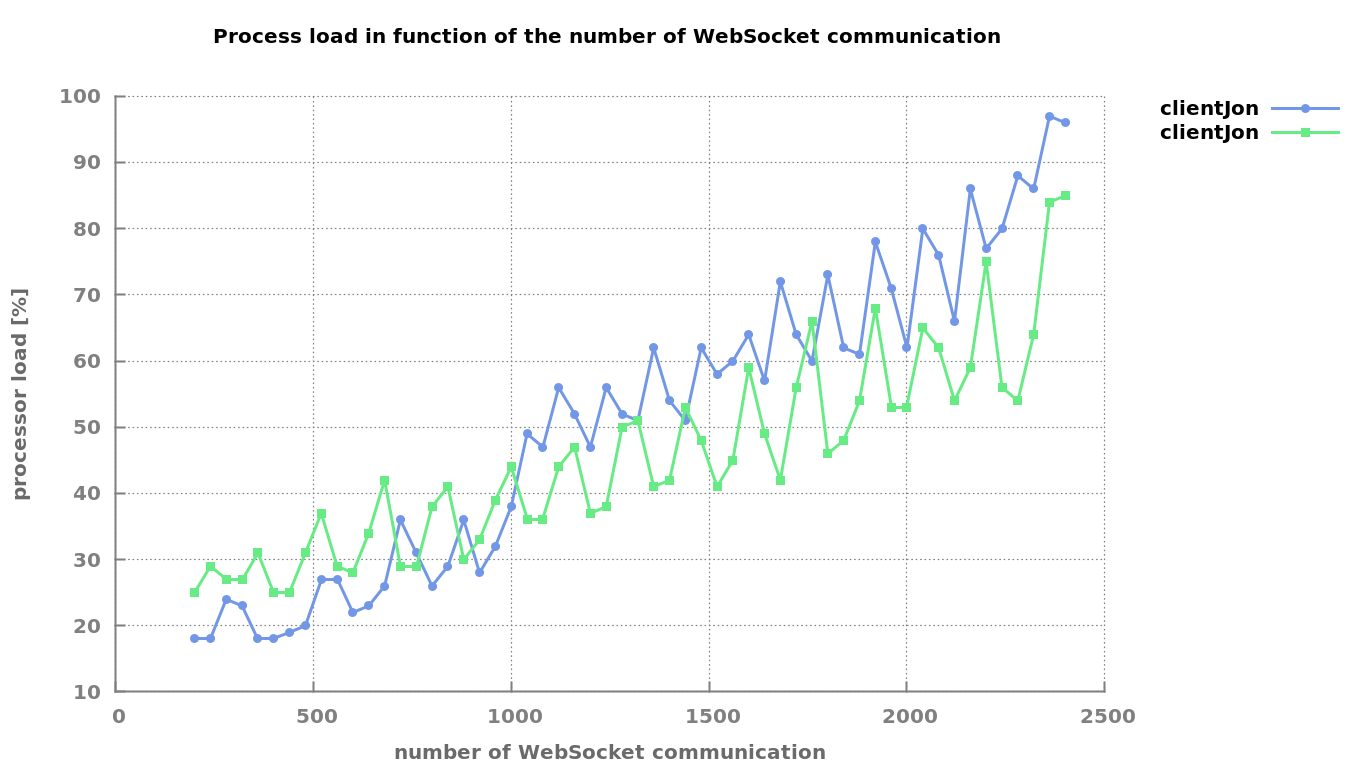
\includegraphics[width=.9\textwidth]{./Figures/WS_client_comparaison.png}
		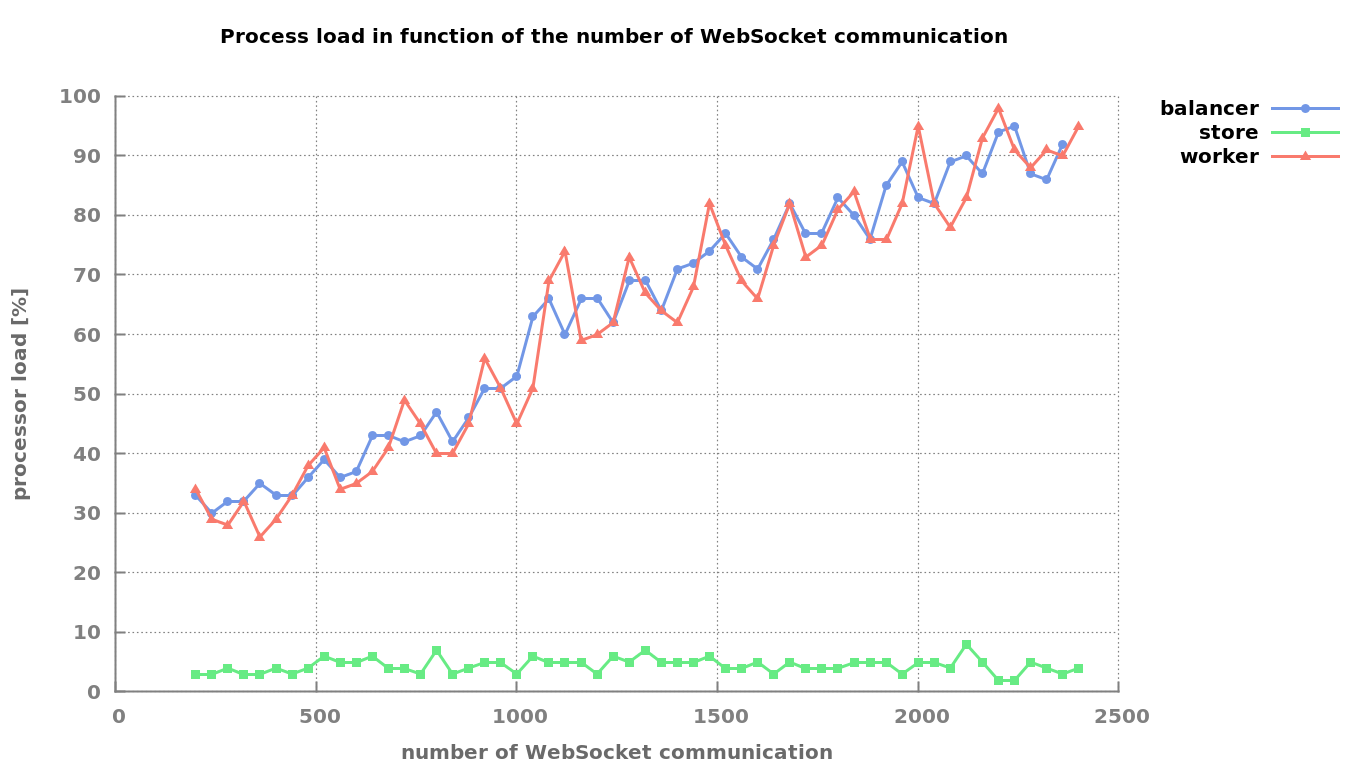
\includegraphics[width=.9\textwidth]{./Figures/WS_server_comparaison.png}
	\caption[WebSocket implementation]{WebSocket implementation}
	\label{fig:WS_comparaison}
\end{figure}

In this experience, two clients are used to achieve a maximum of 2400 WebSocket
communications.  The server was configured to use one storage, one load
balancer and one worker. While the store processor is quite idle, the two other
processors on the other hand are almost used at full capacity.

\textbf{Engine.io implementation}
\begin{figure}[H]
	\centering
		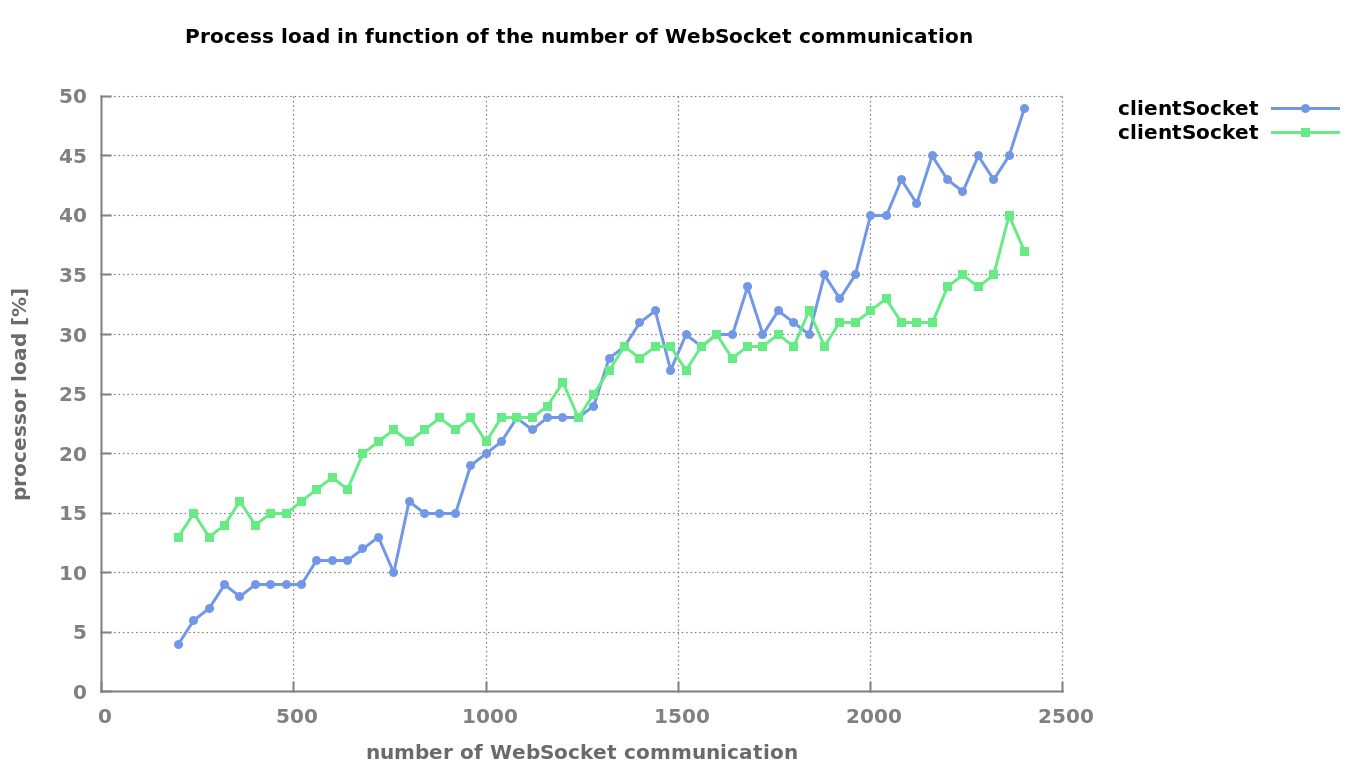
\includegraphics[width=\textwidth]{./Figures/engine_client_comparaison.png}
		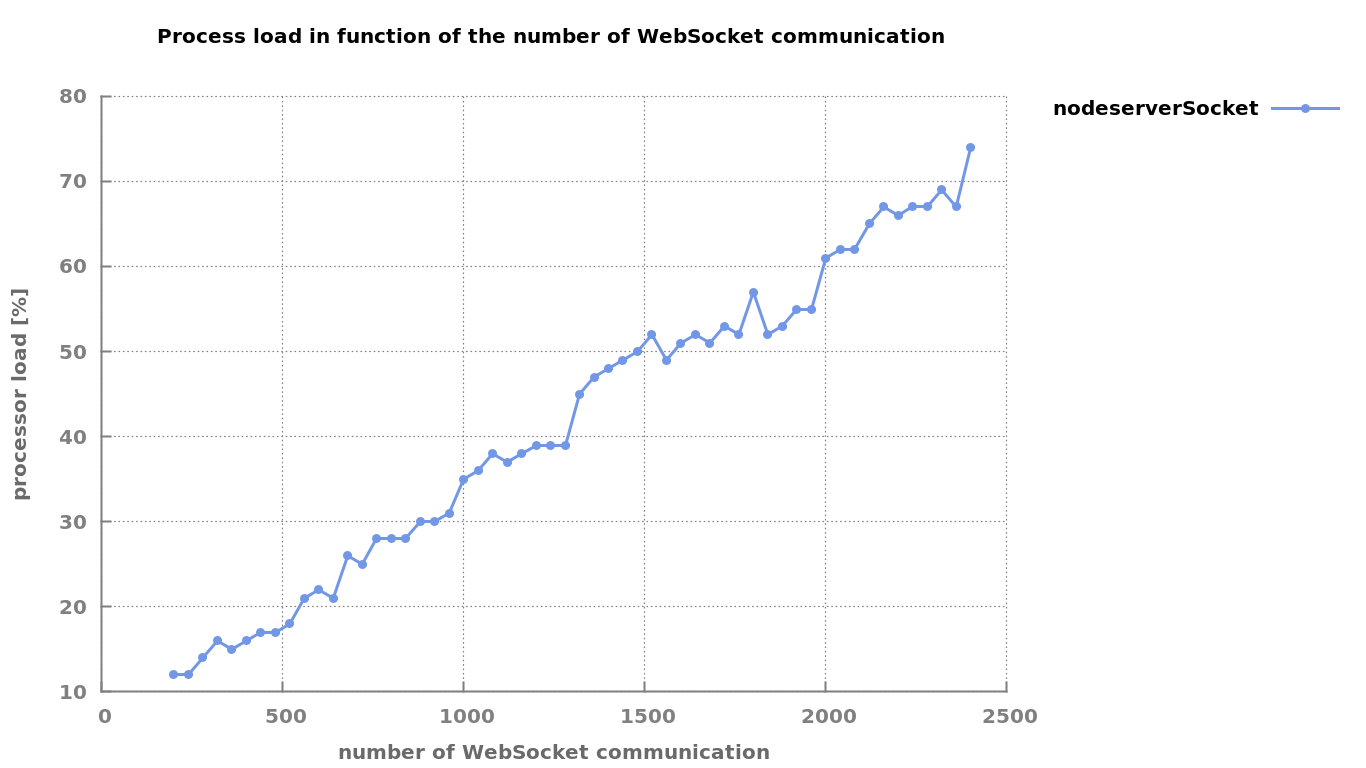
\includegraphics[width=\textwidth]{./Figures/engine_server_comparaison.png}
	\caption[Engine.io implementation]{Engine.io implementation}
	\label{fig:engine_comparaison}
\end{figure}

Surprisingly, pure engine.io implementation seems to be more efficient. Clients
are hitting a maximum of 50\% processor usage compared to 90\% for WebSockets.

On the server side, engine.io processor peaks at 75\% compared to almost
100\% for WebSockets. Also even if both code have been deployed on similar
virtual machines: \texttt{amazon ec2 m3.2xlarge} the engine.io server is
running only on one core compared to three for SocketCluster (one storage,
one load balancer and one worker). This seems to show, SocketCluster is not
adapted to low number of communication.

An interesting study worth doing at this point, is to try to use
SocketCluster on one core.

% -------------
% Third section
% -------------

\section{SocketCluster context switching}

For this experiment a single core  virtual machine is used for the server:
\texttt{amazon ec2 m3.medium}.

\begin{center}
  \begin{tabular}{ | l | l |}
  \hline
  \multicolumn{2}{|c|}{Parameters} \\
  \hline
    Server instance type &  amazon ec2 m3.medium\\ 
    Client instance type &  amazon ec2 m3.2xlarge\\
    Experiment time & 80 s \\
    Number of new communication created at each iteration & 40 \\
    Client creation period & 1 s \\
    Type of ping & random number \\ 
    Ping period & 2.5 s \\ 
    Number of clients & 2 \\
  \hline
  \end{tabular}
\end{center}

\begin{figure}[H]
	\centering
		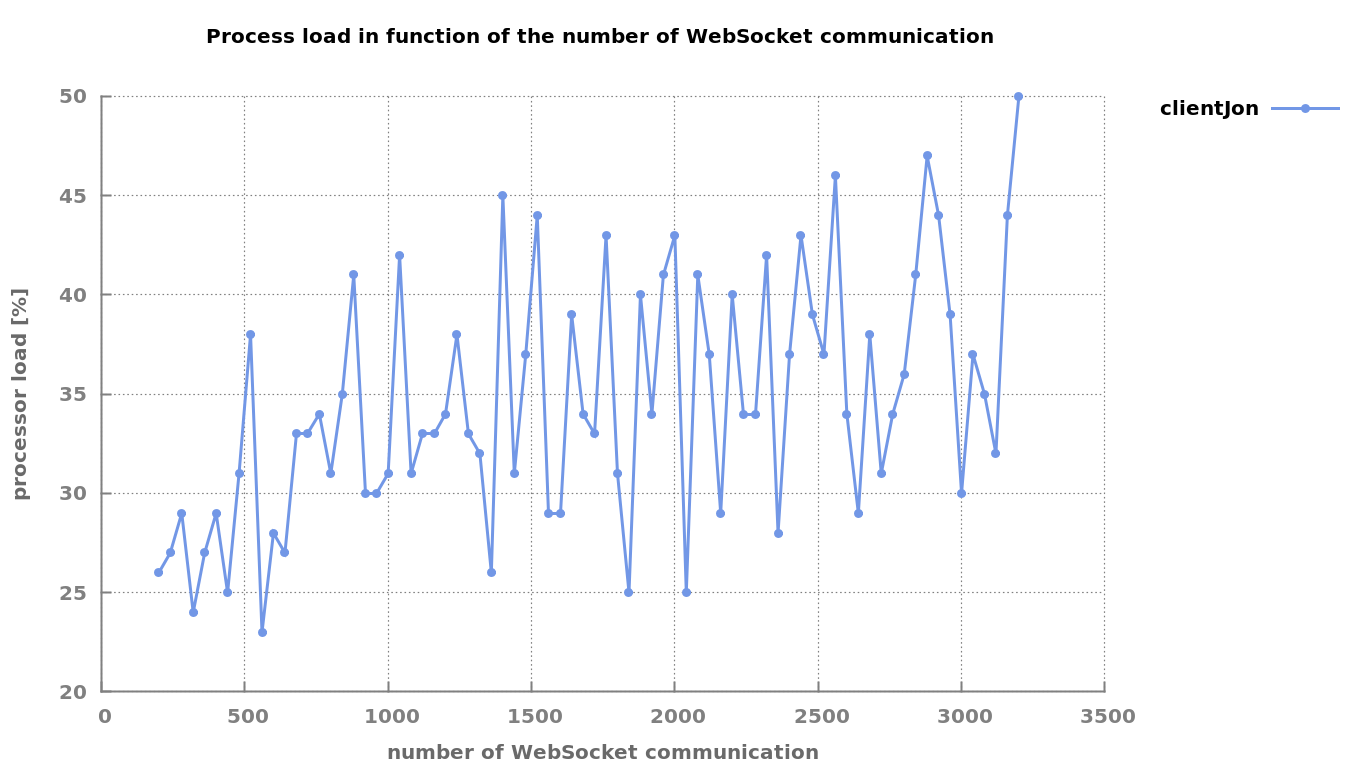
\includegraphics[width=\textwidth]{./Figures/WS_client_context.png}
		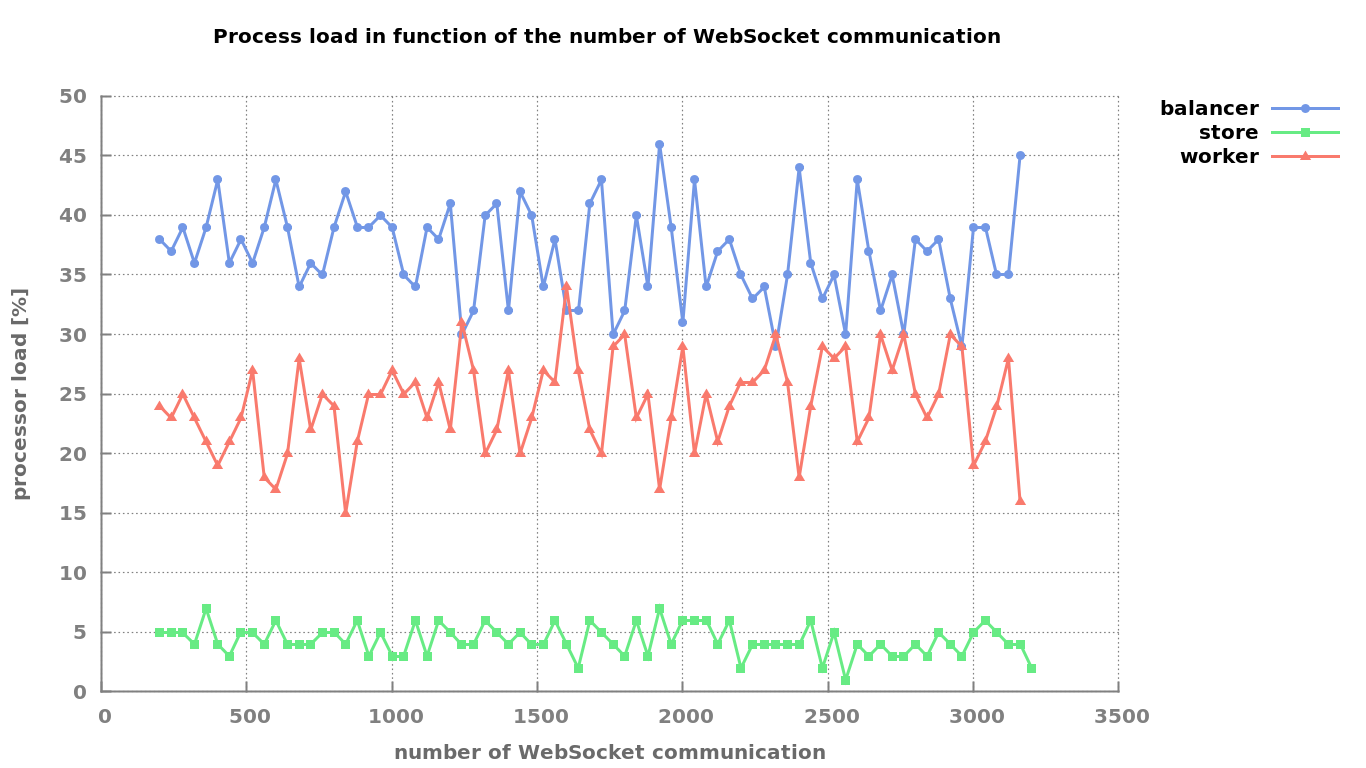
\includegraphics[width=\textwidth]{./Figures/WS_server_context.png}
	\caption[Context switching]{Context switching}
	\label{fig:context}
\end{figure}

At first glimpse, anyone can immediately tell there is a problem with the server
graph. The Load seems to vary randomly at an average of 40\%. What really happens, is
that most WebSocket connections are dropped shortly after being created or they 
not are even created. The problem is a single core needs to handle four threads. So each
time another application is called the context changes. The result is even worse in the case of 
a multi-processor server, because threads are then balanced between processors. Threads 
are heavy weight units, moving them introduces consequent overheads.

In conclusion, this experiment proves SocketCluster is not aimed to be used with
project which involve more threads than available cores.

% --------------
% Fourth section
% --------------

\section{Horizontal scaling of SocketCluster }

This section evaluates the performances of SocketCluster for a growing number
of processors. 

\textbf{Client code}

The client code used in all this part is the same. Two clients are used to
produce a maximum of 2400 WebSocket communications.


\begin{center}
  \begin{tabular}{ | l | l |}
  \hline
  \multicolumn{2}{|c|}{Parameters} \\
  \hline
    Instance type &  amazon ec2 m3.2xlarge\\ 
    Experiment time & 60 s \\
    Number of new communication created at each iteration & 20 \\
    Client creation period & 1 s \\
    Type of ping & random number \\ 
    Ping period & 2.5 s \\ 
    Number of clients & 2 \\
  \hline
  \end{tabular}
\end{center}


\begin{figure}[H]
	\centering
		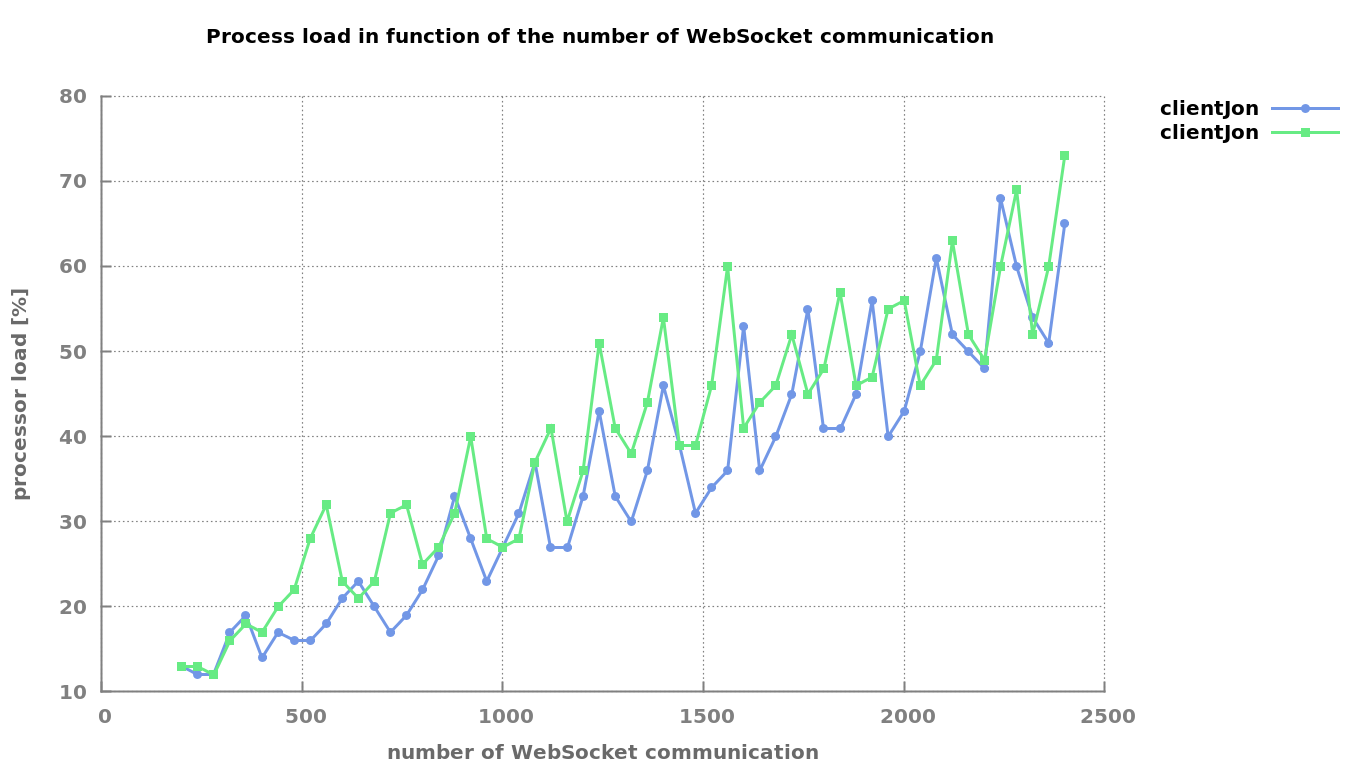
\includegraphics[width=\textwidth]{./Figures/WS_client_rising.png}
	\caption[Simple WebSocket client]{client code}
	\label{fig:WS_client_rising}
\end{figure}

\textbf{Experiment on three cores}

The first test is run a server using a one store, one load balancer and one
worker.

\begin{figure}[H]
	\centering
		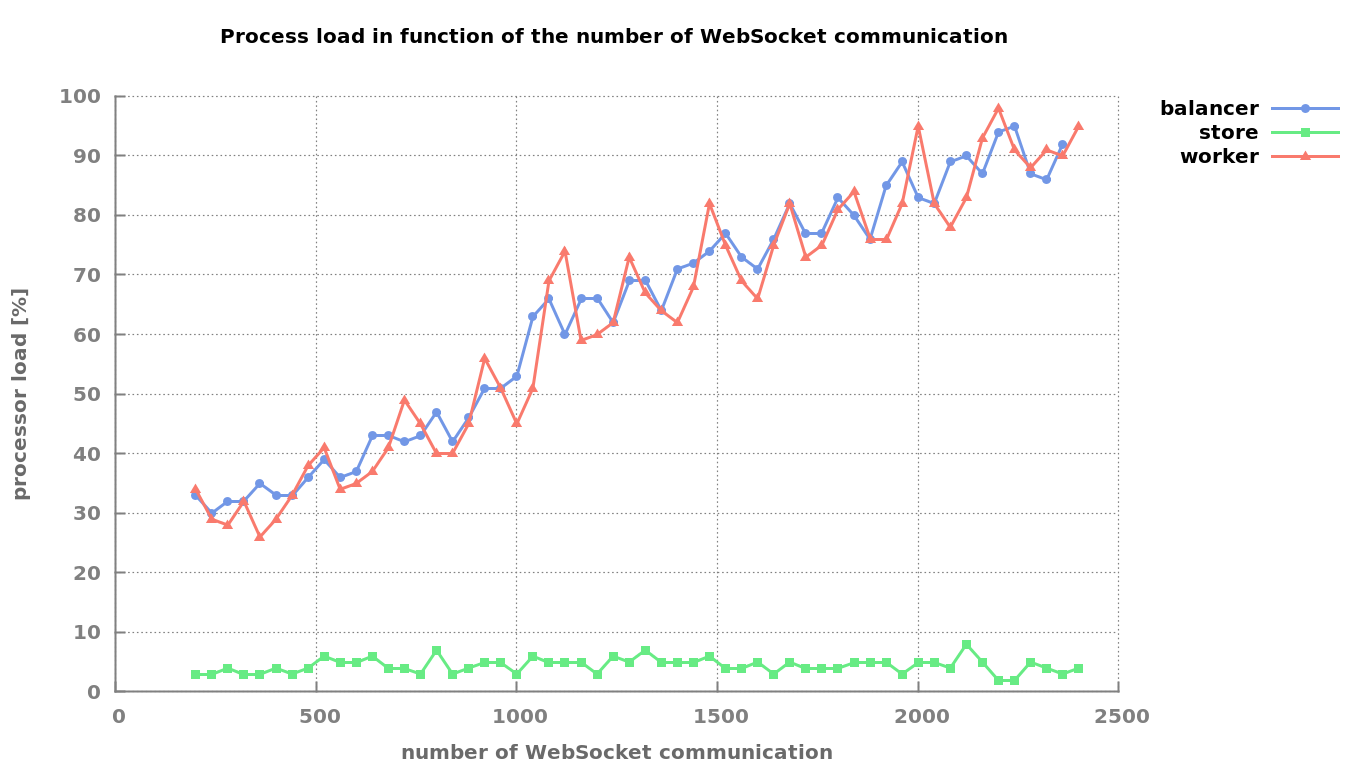
\includegraphics[width=\textwidth]{./Figures/WS_server_1rising.png}
	\caption[WebSocket server on three cores]{Server with three cores}
	\label{fig:WS_server_1rising}
\end{figure}

Figure \ref{fig:WS_server_1rising} clearly shows the worker and load balancer
cores are almost used to their full extent. In order to handle more communication more
cores should be added. 

\textbf{Experiment on five cores}

\begin{figure}[H]
	\centering
		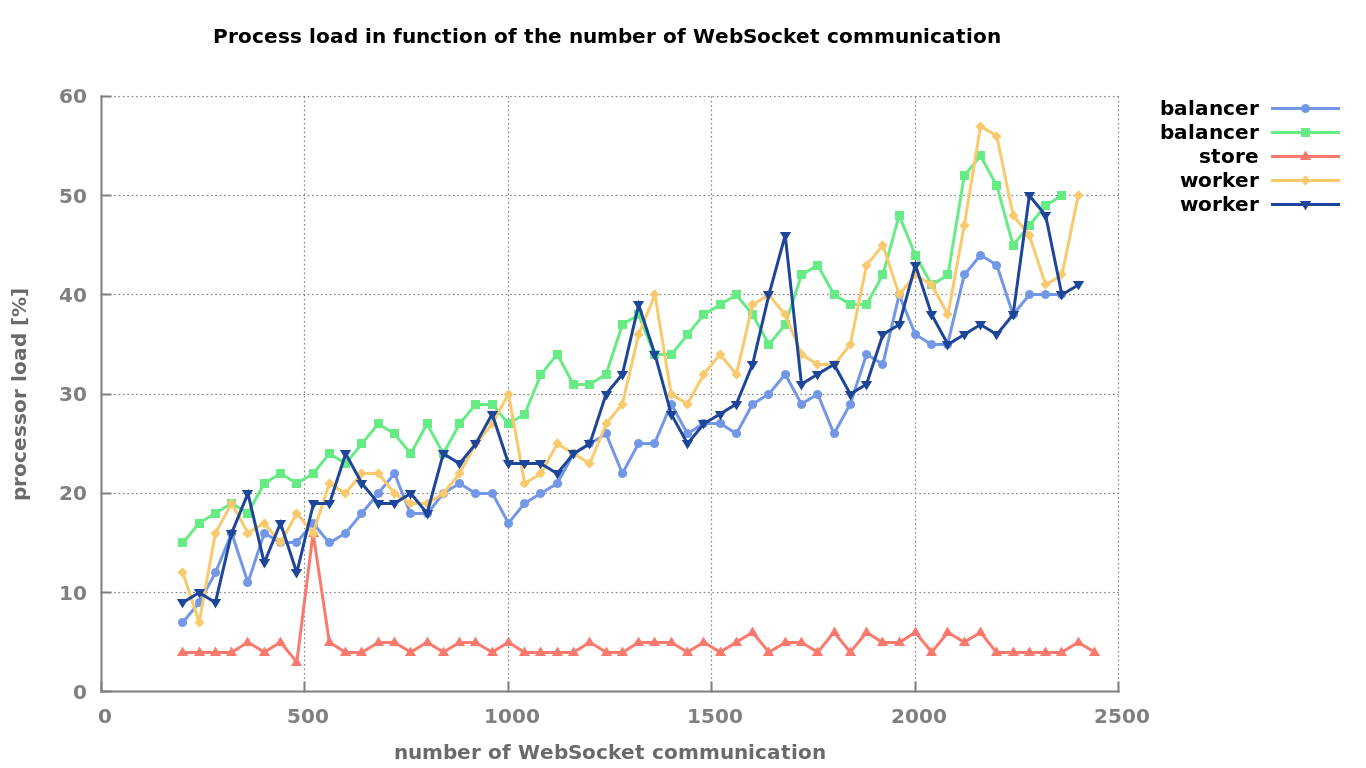
\includegraphics[width=.9\textwidth]{./Figures/WS_server_2rising.png}
	\caption[WebSocket server on five cores]{server with five cores}
	\label{fig:WS_server_2rising}
\end{figure}

In this experiment two more cores have been added. Load balancers and
workers nicely balance the work between themselves and the maximum load drops to 50\%.\\

\textbf{Experiment on seven cores}

\begin{figure}[H]
	\centering
		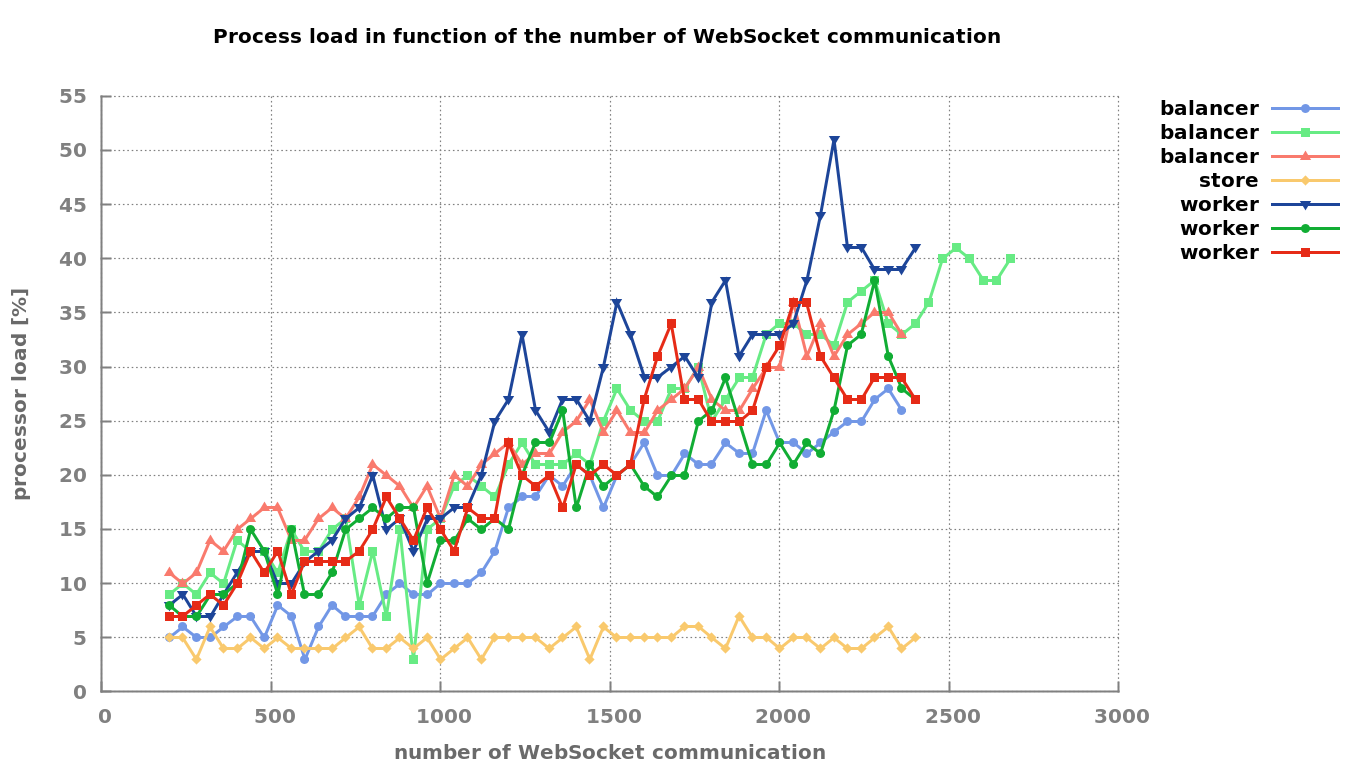
\includegraphics[width=\textwidth]{./Figures/WS_server_3rising.png}
	\caption[WebSocket server on seven cores]{server with seven cores}
	\label{fig:WS_server_3rising}
\end{figure}

This last test is less conclusive. With a total of 3 cores for load balancers
and three for workers the processors load varies between 30\% and 50\%
depending on the task.

As expected, in the long run by adding more processor SocketCluster's
performance get better then engine.io. However in case n is the number of
available processor, SocketCluster is not n times more effective then
engine.io.

\newpage

Actually in this experiment it seems that an equivalent number of workers and
load balancers are needed for the application to run seamlessly. In case the
application doesn't use a store, to gain twice as much computational power, twice
as many processor are required. This makes SocketCluster $\frac{n}{2}$ time
more efficient then engine.io.

Furthermore, it showed adding too many cores is a waste of resources. This
stresses the importance of finding a load balancer/worker/store ratio rule.

% -------------
% Fifth section
% -------------
\section{Parameters' influence}

This section aims at determining which parameter between the number of
WebSocket communications, the period of the pings and the size of the message
exchanged has the most influence on the server processor usage. 

The library \texttt{delivery} has been used to transfer file over WebSocket.
The code can be found in Appendix \ref{fig:WS_server_delivery}.

\begin{center}
  \begin{tabular}{ | l | l |}
  \hline
  \multicolumn{2}{|c|}{Fixed parameters} \\
  \hline
    Instance type &  amazon ec2 m3.2xlarge\\ 
    Experiment time & 60 s \\
    Number of new communication created at each iteration & 20 \\
    Client creation period & 1 s \\
    Type of ping & random number \\ 
  \hline
  \end{tabular}
\end{center}

\newpage

\textbf{Reference experiment}

This first experience will be taken as a reference for the next ones. It has
been carried out with 2 clients establishing together a total of 2400
communications. The period of the pings is in average four seconds and the
size of the file exchanged is 81 bytes.

\begin{figure}[H]
	\centering
		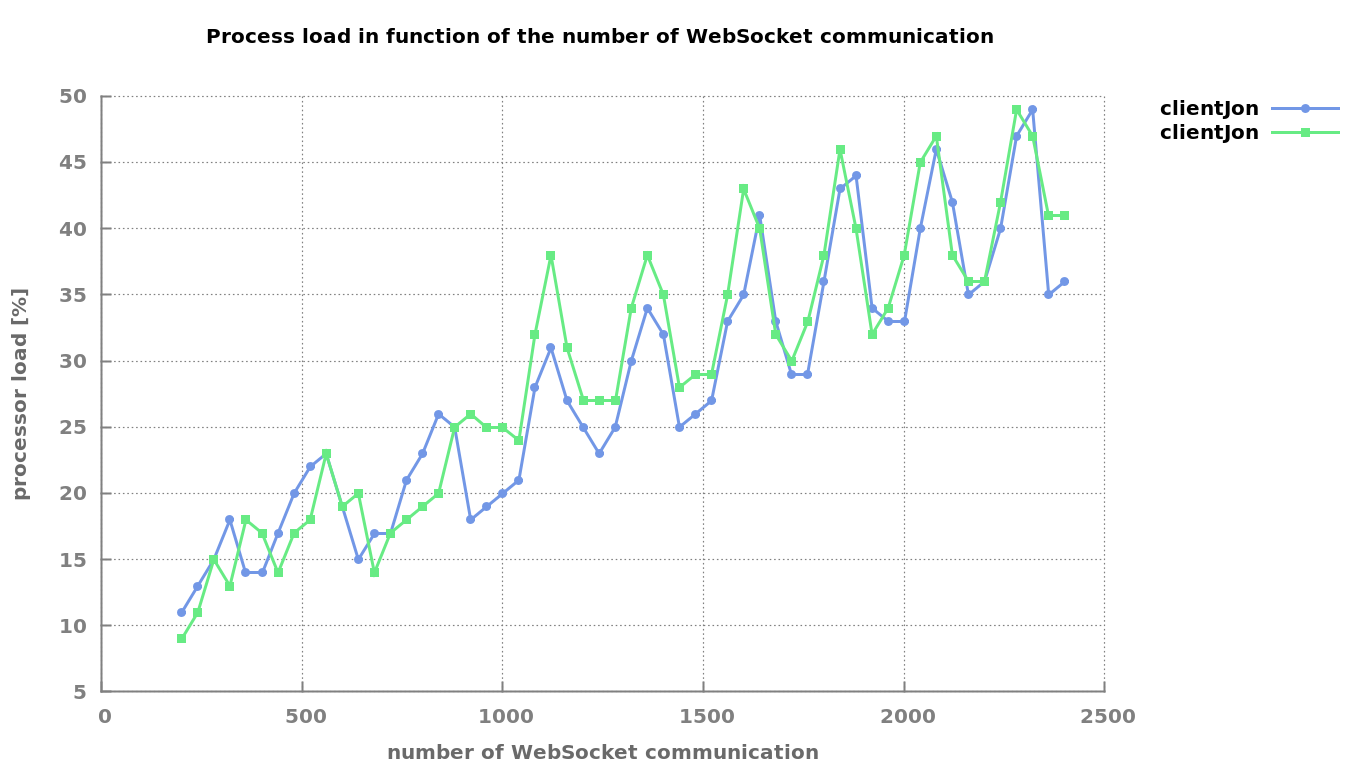
\includegraphics[width=\textwidth]{./Figures/base_client_influence.png}
		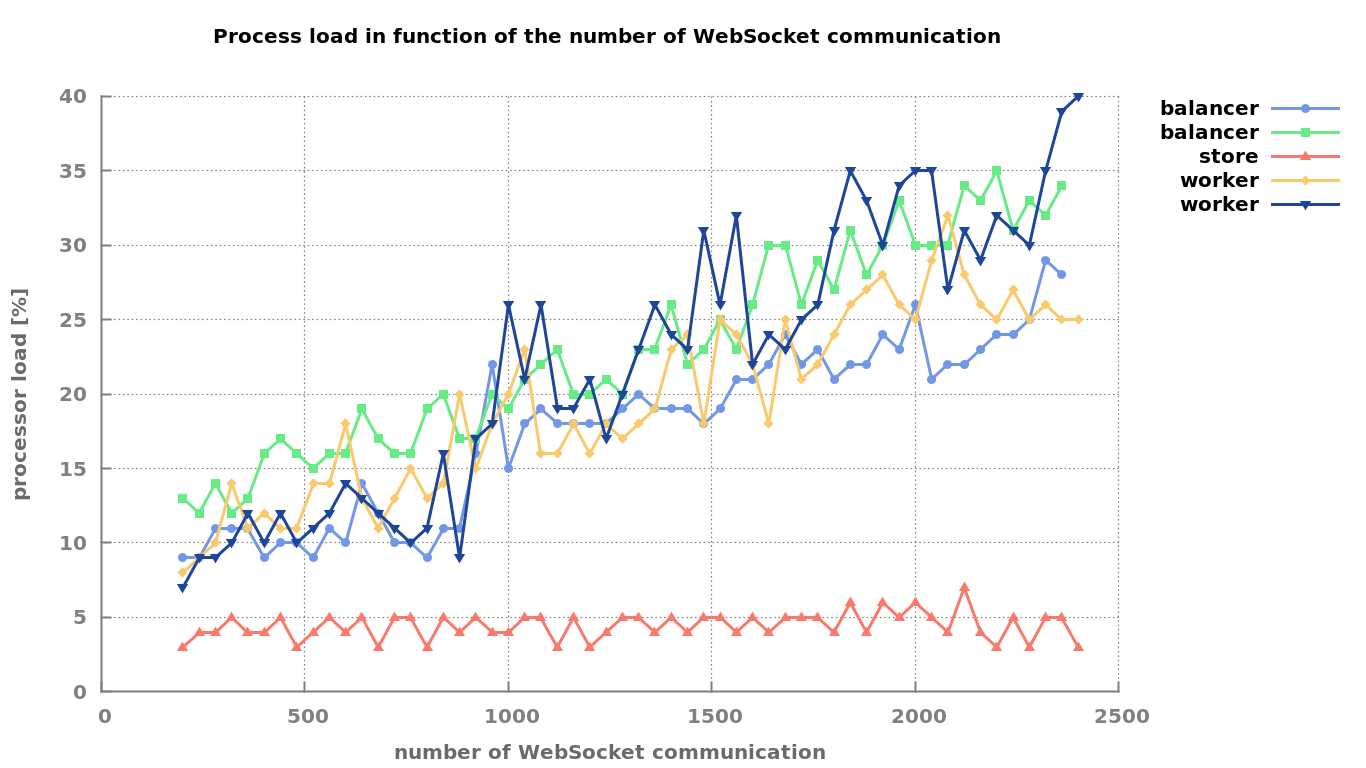
\includegraphics[width=\textwidth]{./Figures/base_server_influence.png}
	\caption[Reference experiment]{Reference experiment}
	\label{fig:base_influence}
\end{figure}

\newpage

\textbf{Pings' period experiment}

In this experiment, the average time separating two pings has been decreased
from four to three seconds.

\begin{figure}[H]
	\centering
		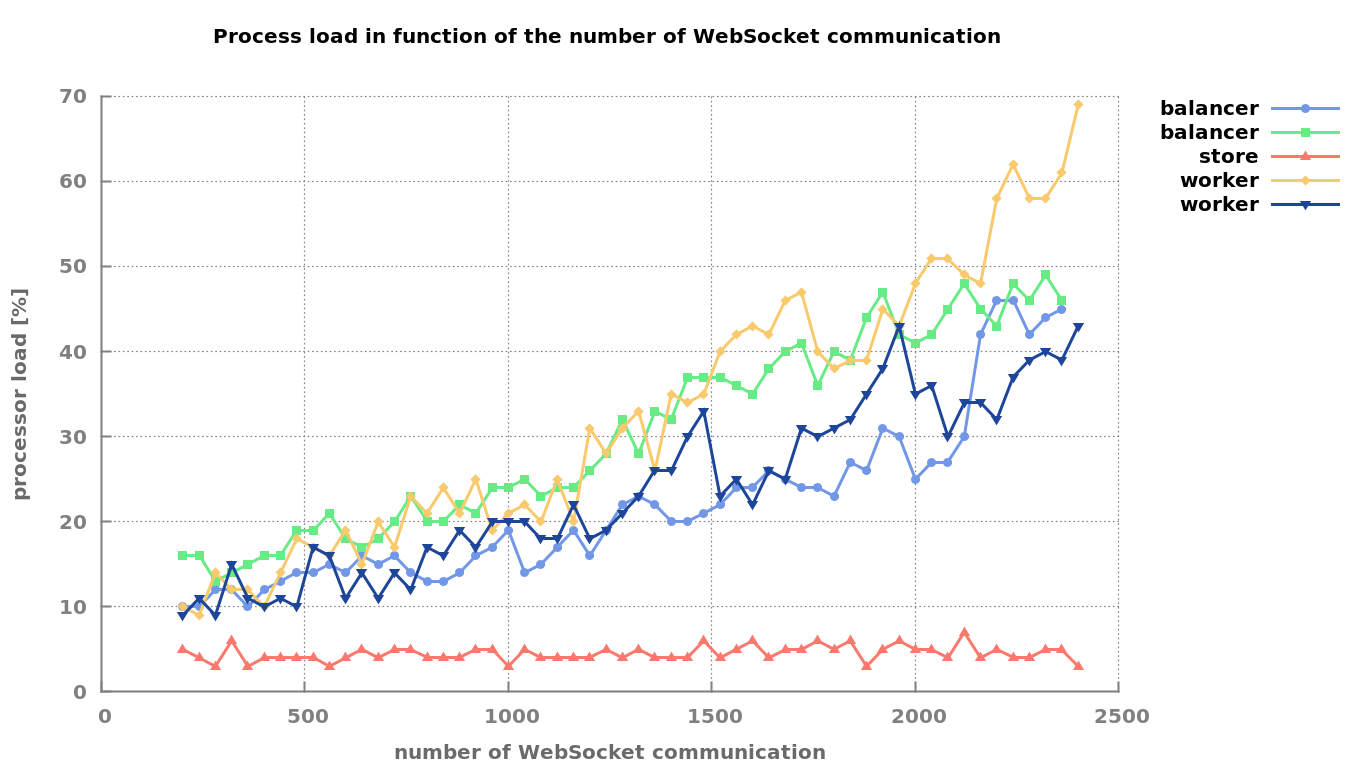
\includegraphics[width=.9\textwidth]{./Figures/ping_server_influence.png}
	\caption[Pings' period experiment]{Pings' period experiment}
	\label{fig:ping_server_influence}
\end{figure}

\textbf{Amount of WebSocket communication experiment}

The following Figure stresses the influence of the number of WebSocket communication
channel. To obtain more communication, a third client has been added compared to 
the reference experience \ref{fig:base_influence}.

\begin{figure}[H]
	\centering
		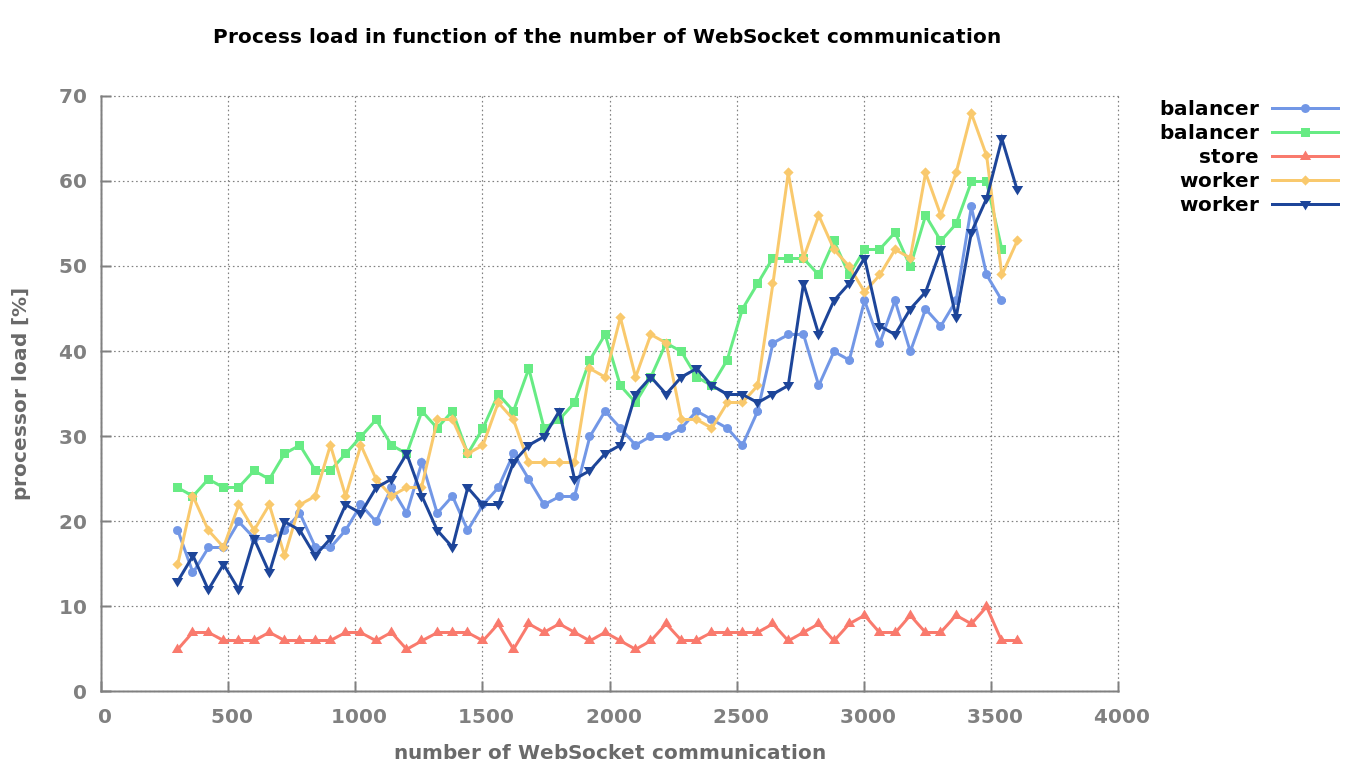
\includegraphics[width=.9\textwidth]{./Figures/communication_server_influence.png}
	\caption[Amount of WebSocket communication experiment]{Amount of WebSocket communication experiment}
	\label{fig:communication_server_influence}
\end{figure}

\textbf{Size of exchanged files experiment}

This last graph underlines the influence of the size of files. The file transferred in this experiment is
500 kbytes compared to 1 kbytes for the reference experience.

\begin{figure}[H]
	\centering
		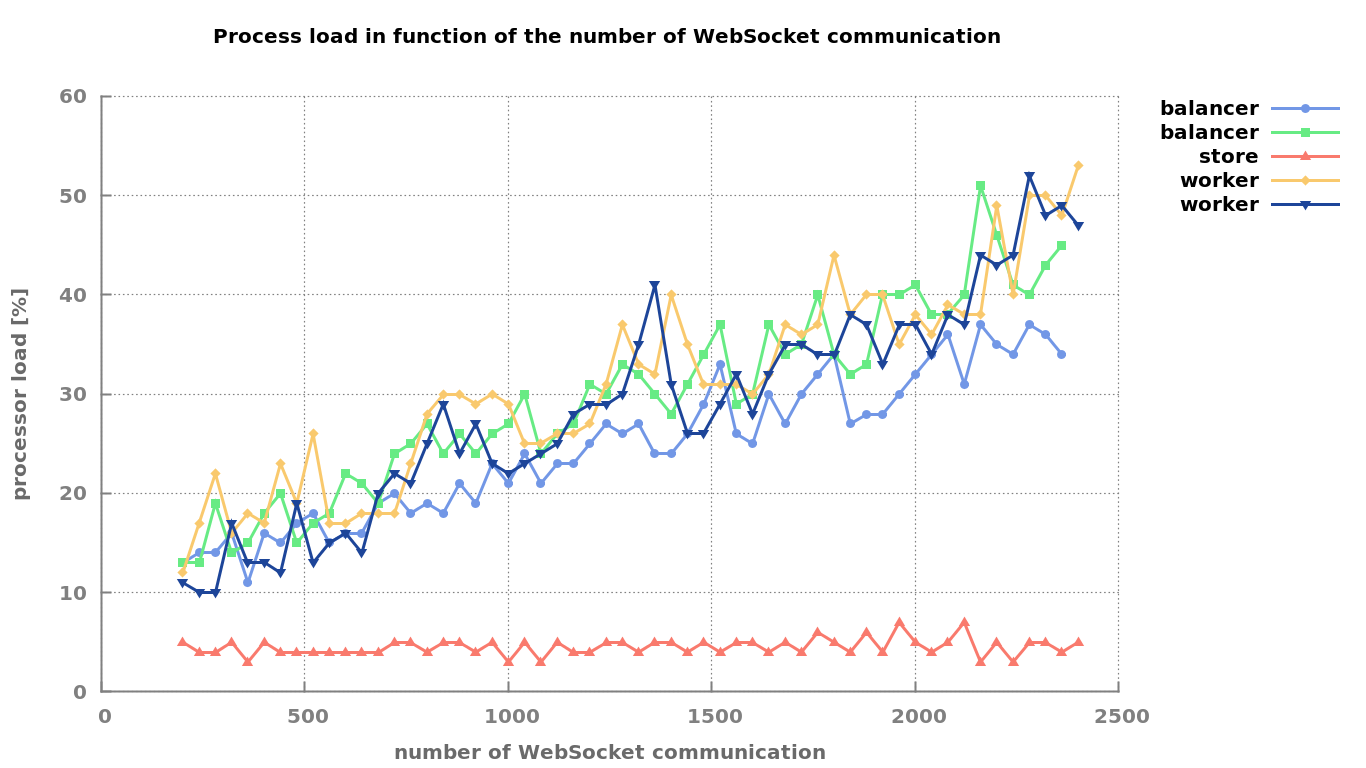
\includegraphics[width=\textwidth]{./Figures/file_server_influence.png}
	\caption[File size experiment]{File size experiment}
	\label{fig:file_server_influence}
\end{figure}


In conclusion, it seems that the size of the exchanged files isn't as important
as the rate of pings and the number of WebSockets communications.

% -------------
% sixth section
% -------------

\section{Concurrent connections experiment}

This study was done to investigate the number of connections a
single server can handle. As seen in the previous section, the number of
connections is tightly bound to the parameters used to simulated the clients
interactions with the server.  Lets suppose each client receives a small file
from the server every 2.5 seconds in average.

\begin{center}
  \begin{tabular}{ | l | l |}
  \hline
  \multicolumn{2}{|c|}{Parameters} \\
  \hline
    Server instance type &  amazon ec2 c3.8xlarge\\ 
    Client instance type & amazon ec2 c3.4xlarge\\
    Experiment time & 150 s \\
    Number of new communication created at each iteration & 10 \\
    Client creation period & 1 s \\
    Ping period & 6 s \\ 
    Size of the file exchanged & small \\
  \hline
  \end{tabular}
\end{center}


\begin{figure}[H]
	\centering
		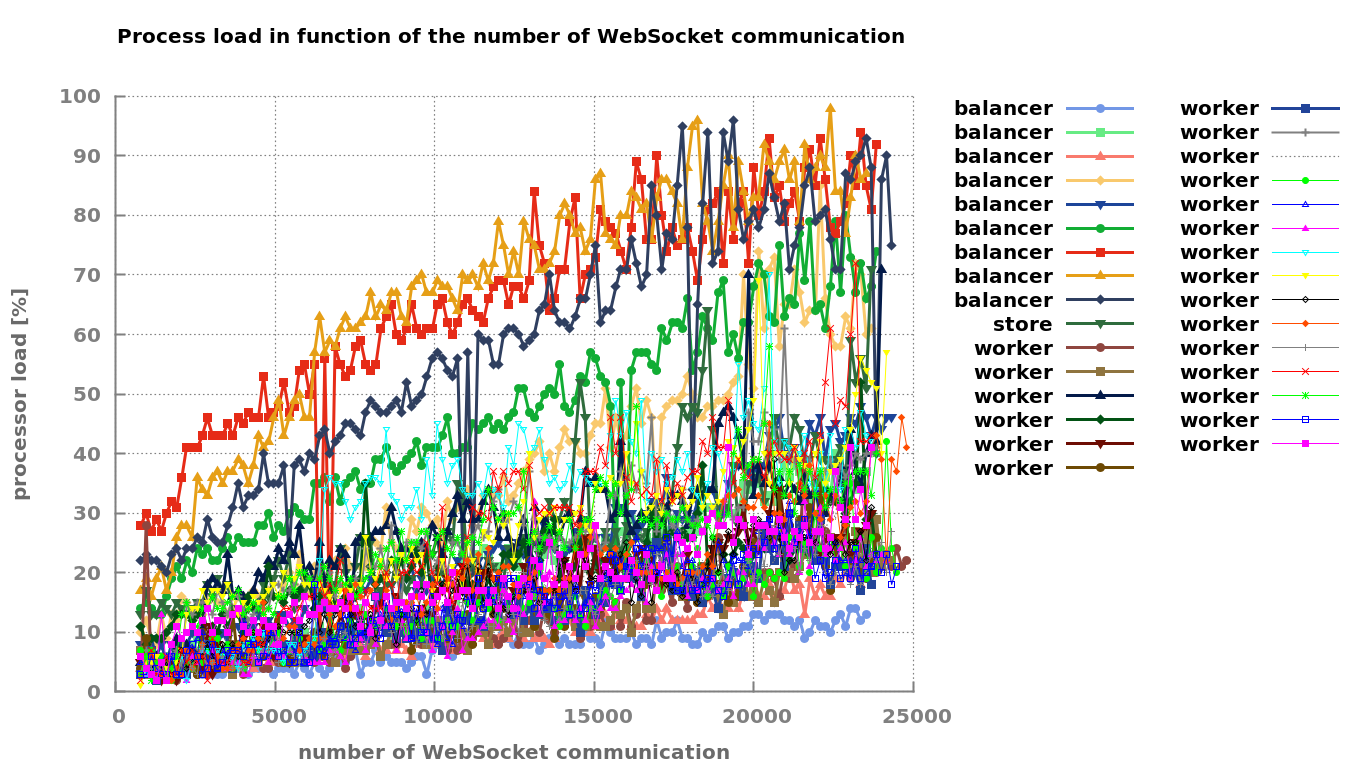
\includegraphics[width=\textwidth]{./Figures/9balancer.png}
		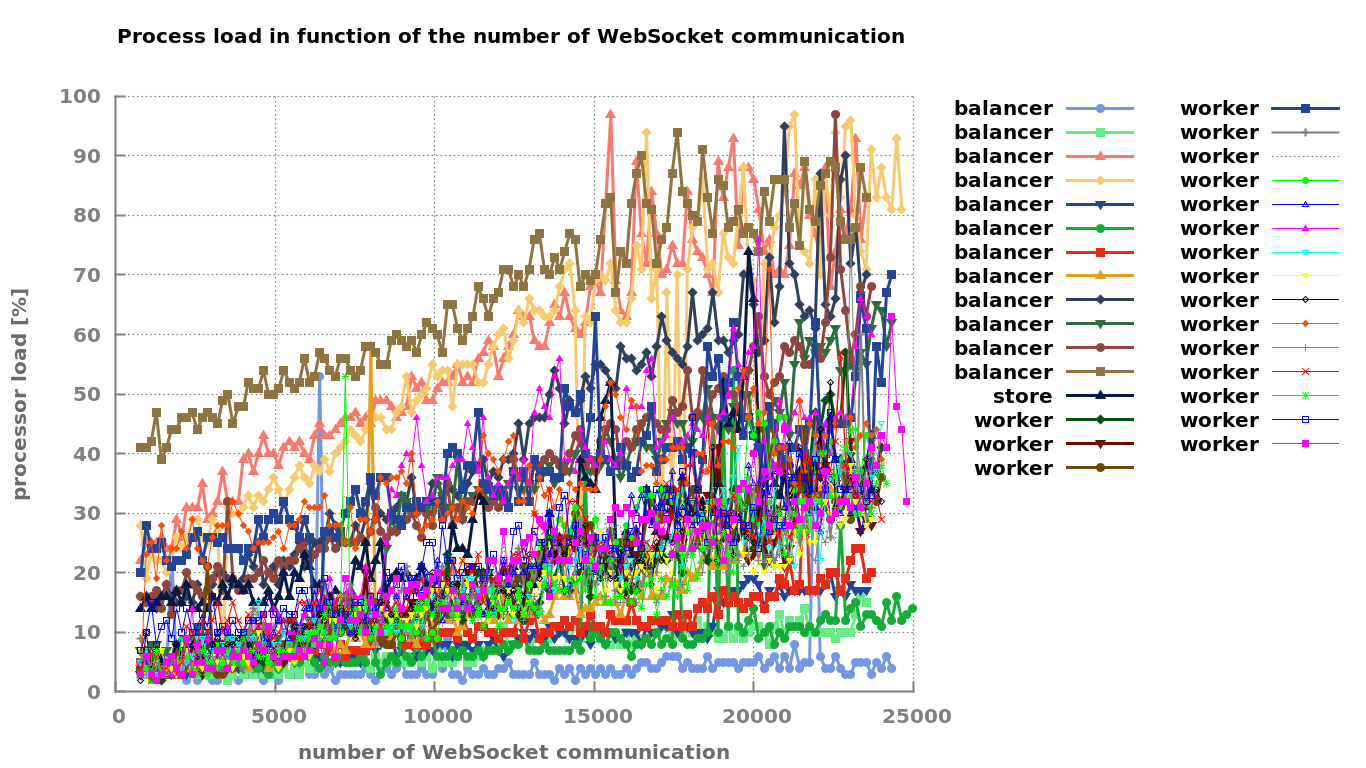
\includegraphics[width=\textwidth]{./Figures/12balancer.png}
	\caption[Maximum number of WebSocket communication]{Maximum number of WebSocket communication}
	\label{fig:max_communication}
\end{figure}

This experiment has been carried out on the biggest server made available by
amazon ec2.  SocketCluster will hardly be used in this conditions during normal
usages.  It is way cheaper to make clusters of SocketClusters server then to
use a beastly server like this one.

This experiment confirmed SocketCluster is able to support around 25 000
concurrent connections. It also pointed out an imperfection of SocketCluster.
The first graph is an experiment with 9 load balancers and 21 workers. The
second with 12 load balancers and 18 workers.  In the first experiment the load
balancers' load is quite high. Adding more communication will result in
communication to be dropped, as a result the second experiment has been carried
out with more load balancers. But the previous figures clearly show that some
load balancer are still using way too much computing power and some on the
other hand are almost idle.

This points out a bad load balancing between the load balancers themselves.

\section{Experiment summary}

The client throughout tests showed the number of communications are scaling
linearly when adding more cores. It also gave an insight into the user
experience when using SocketCluster.

The second section was a little disappointing, one would expect a SocketCluster
code running on three cores to achieve better then a regular engine.io code
running on one core. However it is not the case, engine.io is significantly
better.

The third section stresses the importance of running SocketCluster on a less
processus then available cores. Otherwise the operating system as to operate
heavy weight context switching.

The forth section studies the horizontal scaling of SocketCluster. Apparently,
in a relatively low parallel environment, the application needs as much
load-balancers as worker. And once they get saturated, adding a load-balancer
and a worker will efficiently increase the performances.

The fifth experiment demonstrated the number of communication and the periods
of pings increase the processor usage more quickly then the size of the
messages exchanged.

The last experiment which was intended as a pure concurrent experiment, proved
SocketCluster can handle 25k communications on a single server. But more
importantly it showed that in a highly parallel environment, the load balancers
begin to miss behave.











